\section{Path Smoothing}
It should be noted that all of the path planners covered, in this paper, have generated piece-wise linear paths between two discrete points in space. With the exception of a path that only contains two points, the shortest path generated by these planners will always be discontinuous. The nature of this discontinuity is rooted in the discretization applied earlier throughout these planners. Unfortunately, while discretized paths are computationally desirable, they often are incompatible with the robotics system that will use the planners path.

\begin{figure}[h]
    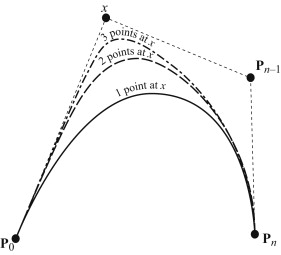
\includegraphics[width=4cm]{cubic_bezier}
    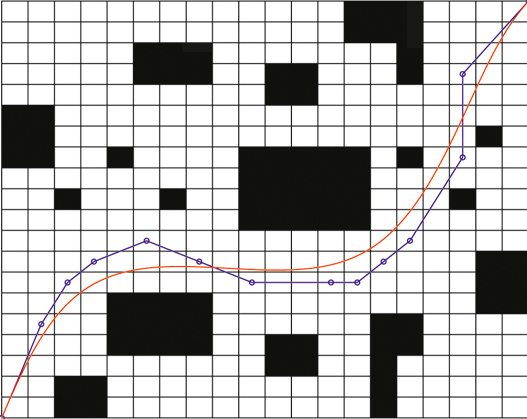
\includegraphics[width=4.5cm]{bezier_path_smoothing}
    \centering
    \label{fig:bezier}
    \caption{Cubic Bezier}
  \end{figure}

The most obvious reason for such an incompatibility is the requirement for continuous inputs into a controller, state estimator, or other component which are formulated under the assumption of continuous inputs. Secondly, even for discrete systems, it is often more desirable to generate waypoints, for the robot to track, at a much higher sampling frequency, than is practicable to produce with the planner directly. This is especially true when refining the discretization of the map to a sufficient waypoint frequency would make global path planning through the environment untractable.

This need leads to the need for the raw outputs of these planners to be post-processed via a path smoothing algorithm. As alluded to above, in this paper, the reason for smoothing the outputs of the planner come from desiring a frequency between waypoints.

\subsection{Bezier Path Smoothing}
One of the most simple and straight forward methods for path smoothing is that of Bezier curves. While the derivation of Bezier curves is beyond the scope of this paper, sufficed to say that this technique is very effective for quickly computing a curve from the planner output, that is effectively infinitely resolvable.

\subsubsection{Bezier Curve Formulation}
The formulation of a Bezier curve is the based on the three following equations. 

\begin{equation}
    \left(\begin{array}{l}
    n \\
    i
    \end{array}\right)=\frac{n !}{i !(n-1) !}
\end{equation}

\begin{equation}
    B_{i, n}(t)=\left(\begin{array}{c}
    n \\
    i
    \end{array}\right) t^i(1-t)^{n-i}
\end{equation}

\begin{equation}
    C(t)=\sum_{i=0}^n P_i B_{i, n}(t)
\end{equation}

Where $P_i$ is the point at index $i$ from output of the planner which is of length $n$ and where $B_{i, n}$ is formula for a Bernstein polynomial. 

As with the mathematical formulation of the Bezier curve, the implementation of the Bezier,in code, is very direct and straightforward. 

% \begin{figure}[h!]
%     % 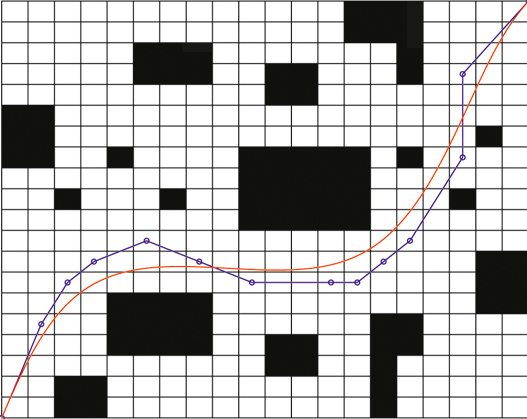
\includegraphics[width=4cm]{bezier_path_smoothing}
%     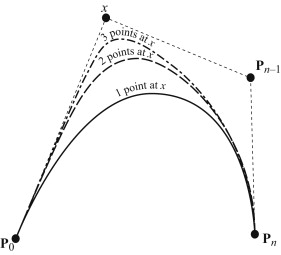
\includegraphics[width=4cm]{cubic_bezier}
%     \centering
%     \label{fig:Bezier_Curves}
%     \caption{Bezier Path Smoothing}
% \end{figure}  


\subsubsection{Limitation of Bezier Curves}
Unless the length of the planner output is exceeding large, Bezier curves tend be a quick to compute path smoothing algorithm that is very effective for many applications including simple robotic environments or in video games. Unfortunately, the primary drawback of Bezier curves in robotics, is the inability to directly model system or environmental information into the path smoothing process. In the domain of robotics, this typically manifests as the inability to apply custom constraints or guarantee feasibility of the final smoothed path.  

While guaranteeing feasibility or respecting applied constraints, might be of little meaningful importance in an application like video games, where the goal is to be good enough while using up the least compute resources, in robotics, obeying constraints and feasibility requirements is a very real necessity.

While not ideal, the Bezier curves does often work for robots in simple environments. Acknowledging this short-coming, this paper, has applied Bezier path smoothing to all of the path planner outputs as a means of quickly and consistently generating a smooth output path.


\subsection{Optimization Based Path Smoothing}
The other predominate class of path smoothing algorithms comes in the form of optimization based methods. Unlike Bezier smoothing, these methods work on the principle of minimizing some cost function associated with the points output by the planner. The strength of optimization-based methods involve the natural ability to define and apply constraints to that the solution of the optimizer must obey. For path smoothing, this translates into the ability for these methods to intuitively constraints such that the smoothed path will never intersect with static obstacles in the environment, or violate feasibility by generating a path whose curvature is impossible for the robot to track.

Generally, this method is far more computationally expensive to realize than that of Bezier curves; however, the benefits that it brings are often significant enough for specialize high efficiency variants to be designed specially for real-time robotic applications. 

\subsubsection{Timed-Elastic Band}
One such method that has been specially adapted for the use with car-like robots (e.g. autonomous vehicles), is that of \textbf{Timed-Elastic Band} optimization. This problem is formulated mathematical below.  

\begin{equation}
    \begin{array}{l}
    \min _{\mathcal{B}} \sum_{k=1}^{n-1} \Delta T_k^2 \quad(\mathrm{NLP}) \\
    \text { subject to } \\
    \mathbf{s}_1=\mathbf{s}_c, \mathbf{s}_n=\mathbf{s} f, 0 \leq \Delta T_k \leq \Delta T_{\max }, \\
    \mathbf{h}_k\left(\mathbf{s}_{k+1}, \mathbf{s}_k\right)=0, \quad \tilde{r}_k\left(\mathbf{s}_{k+1}, \mathbf{s}_k\right) \geq 0, \\
    \mathbf{o}_k\left(\mathbf{s}_k\right) \geq 0, \\
    \nu_k\left(\mathbf{s}_{k+1}, \mathbf{s}_k, \Delta T_k\right) \geq 0, \quad(k=1,2, \ldots, n-1) \\
    \alpha_k\left(\mathbf{s}_{k+2}, \mathbf{s}_{k+1}, \mathbf{s}_k, \Delta T_{k+1}, \Delta T_k\right) \geq 0,(k=2,3, \ldots, n-2) \\
    \alpha_1\left(\mathbf{s}_2, \mathbf{s}_1, \Delta T_1\right) \geq 0, \quad \alpha_n\left(\mathbf{s}_n, \mathbf{s}_{n-1}, \Delta T_{n-1}\right) \geq 0 .
    \end{array}
    \end{equation}

The advantage of this algorithm is that it incorporates a standard vehicle model and produces locally optimal paths. The downside of this method is that it is required to be run online, very similarly to the implementation of Model Predictive Control (MPC).



